\documentclass[a4paper,12pt,titlepage]{article}
\usepackage[utf8]{inputenc}
\usepackage{graphicx} % Required for inserting images
\usepackage[spanish,es-tabla]{babel}
\usepackage[none]{hyphenat}
\usepackage[justification=centering]{caption}
\usepackage{subcaption}
\usepackage{amssymb, amsmath}
\usepackage{gensymb}
\usepackage{fancyhdr}
\usepackage{longtable}
\usepackage{wrapfig}


\lhead{Bobinas Helmholtz}
\rhead{Gonzalo Bastos González}

\pagestyle{fancy}

\title{Bobinas Helmholtz}
\author{Gonzalo Bastos González}

\begin{document}

\section{Introducción teórica}

El objetivo de esta práctica es medir el campo magnético axial creado por dos bobinas paralelas variando la distancia que las separa. La configuración experimental que vamos a adoptar, conocida como bobinas de Helmholtz, tiene la particularidad de que cuando la distancia que separa a las bobinas es igual a su radio el campo magnético creado por las bobinas en su interior es prácticamente constante, algo que comprobaremos experimentalmente. Esta particularidad hace que las bobinas de Helmholtz sean muy útiles en experimentos en los que se necesita trabajar con campos magnéticos constantes.

\par La expresión del campo magnético creado por las bobinas es la siguiente:

\begin{equation}
    B=\frac{\mu_0 I N}{2 R}\left[\frac{1}{\left(1+\left(\frac{z-a / 2}{R}\right)^2\right)^{3 / 2}}+\frac{1}{\left(1+\left(\frac{z+a / 2}{R}\right)^2\right)^{3 / 2}}\right]
    \label{Campo magnético}
\end{equation}

Las variables de las que depende son:

\begin{itemize}
    \item $\mu_{0} = 4\pi \cdot 10^{-7} \; T\cdot m \cdot A^{-1}$ (Permeabilidad magnética del vacío)
    \item $R= 0,20 \; m$ (Radio de las bobinas)
    \item $a =$ Distancia entre bobinas (m)
    \item $I=$ Intensidad que circula por las bobinas (A)
    \item $N=154$ (Número de espiras)
    \item $z=$ Distancia desde el punto medio del segmento que une los centros de las bobinas, que denominaremos origen de medidas, hasta un punto del eje de las mismas (m)
\end{itemize}


\section{Materiales y metodología}

Los materiales empleados en la práctica son:

\begin{itemize}
    \item Dos bobinas de 20 cm de radio
    \item Fuente de alimentación que proporcionará la intensidad que va a circular por las bobinas
    \item Amperímetro para medir esa intensidad de corriente
    \item Teslámetro con una sonda Hall para medir el campo magnético
    \item Regla y metro rígido para medir las diferentes distancias
\end{itemize}

La disposición empleada se muestra en la siguiente figura salvo una pequeña excepción, nuestra sonda Hall se dispone paralela al eje de las bobinas, por lo que se encuentra situada sobre el eje X de la segunda imagen y de desplazará sobre él para medir los diferentes valores de z.

\begin{figure}[h!]
    \begin{subfigure}{0.6\textwidth}
        \centering
        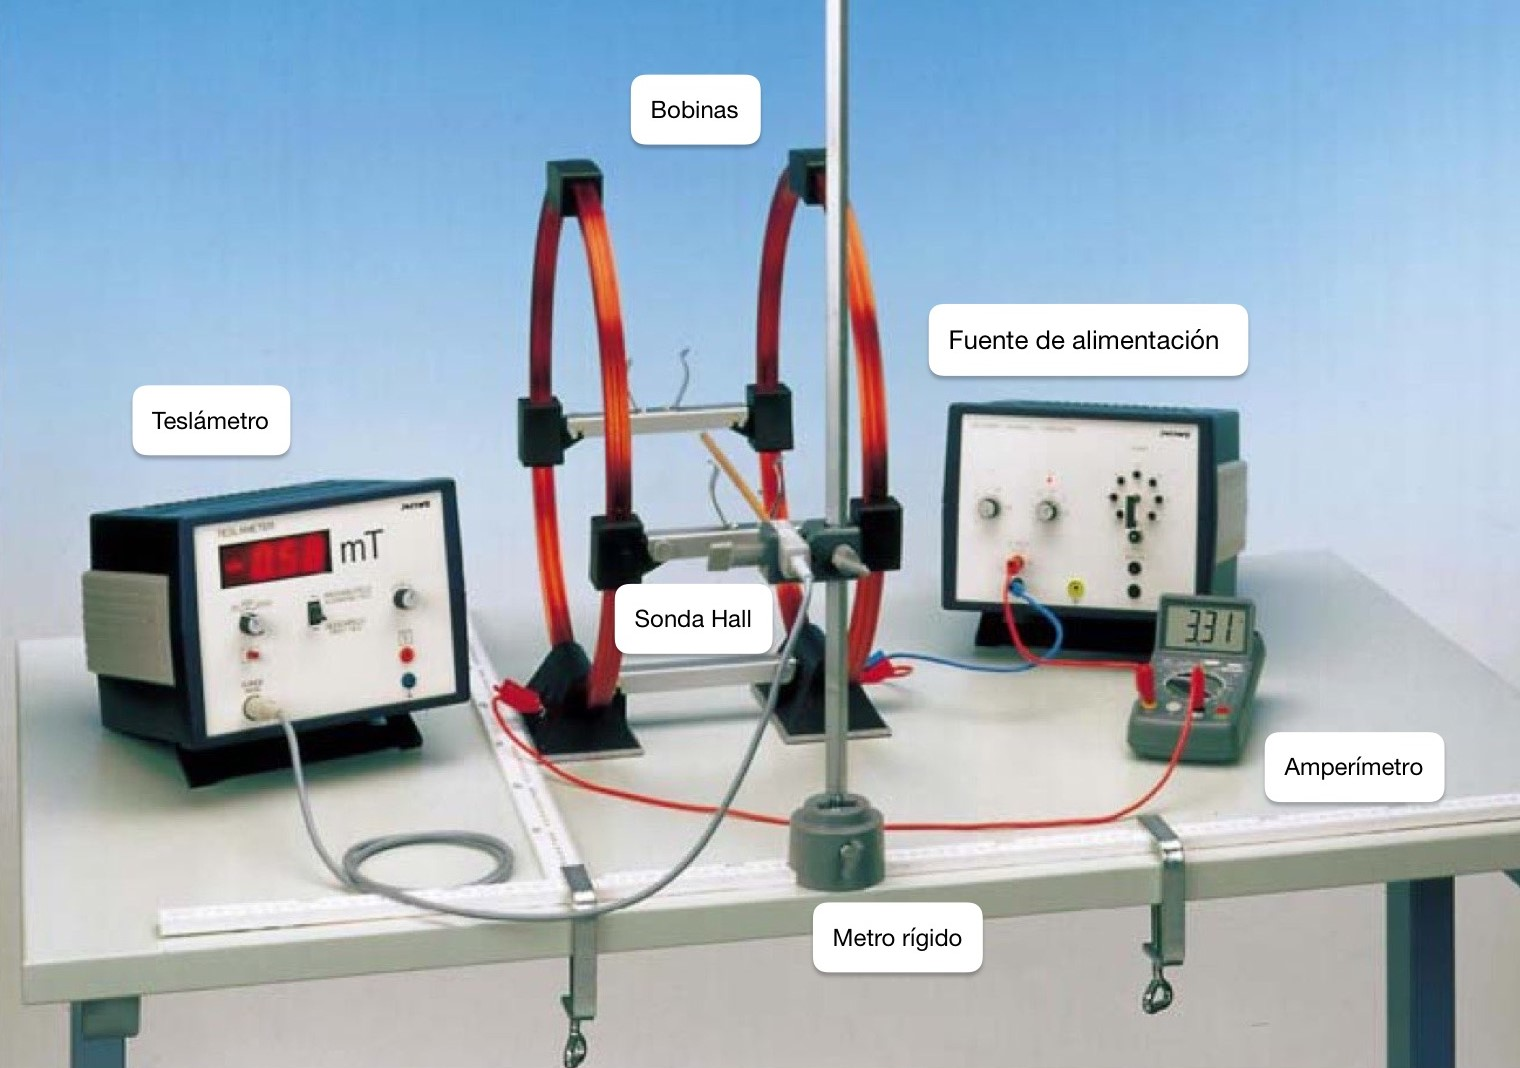
\includegraphics[width=0.95\linewidth]{Images/Bobinas configuración-1.jpg}
    \end{subfigure}
    \begin{subfigure}{0.52\textwidth}
        \centering
        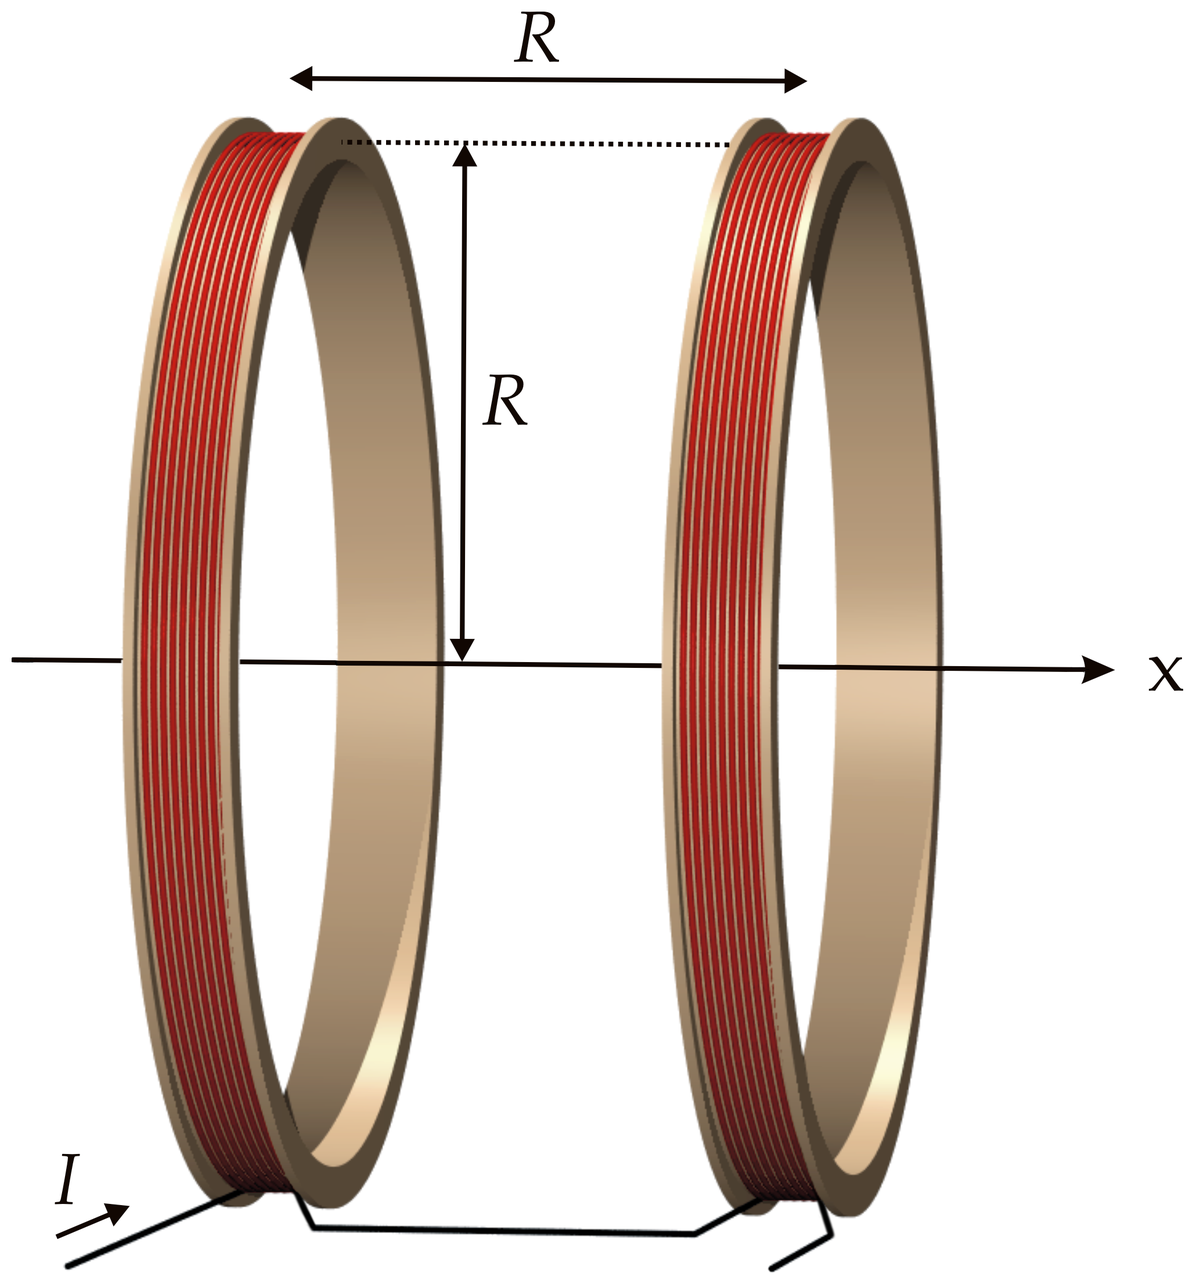
\includegraphics[width=0.75\linewidth]{Images/bobinas esquema.png}
    \end{subfigure}
    \caption{Montaje experimental de las bobinas Helmholtz}
\end{figure}

\par Esta práctica consta de dos partes bien diferenciadas, el estudio del campo magnético axial creado por las bobinas y la determinación de la constante de permeabilidad magnética. La metodología seguida en cada parte se detallará a continuación:

\subsection{Estudio del campo magnético axial}

El objetivo de esta práctica es medir experimentalmente el campo magnético creado por las bobinas a lo largo de su eje, variando las distancias que las separa. Tomaremos medidas en tres situaciones diferentes, variando el valor de $a$, la separación entre bobinas. En primer lugar estudiaremos el campo magnético con $a=R$, luego con $a=2R$ y, por último, con $a=R/2$. Para cada una de estas tres situaciones tomaremos alrededor de 60 valores del valor del campo magnético ($B_{exp}$) frente a diferentes valores de $z$, desplazando la sonda a lo largo del eje, a una intensidad constante de 3 A. Las incertidumbres de los aparatos de medida con los que trabajamos son las siguientes:

\begin{itemize}
    \item La incertidumbre de los valores medidos del campo magnético viene dada por la precisión del teslámetro:
    
    \begin{equation}
        s(B_{exp}) = 0,01\; mT = 10^{-5} \; T
        \label{Inc campo magnético}
    \end{equation}

    \item La incertidumbre de la intensidad viene dada por la precisión de la fuente de alimentación:
    
    \begin{equation}
        s(I) = 0,01 \; A
        \label{Inc intensidad}
    \end{equation}

    \item La incertidumbre de los valores de $z$ la obtendremos de forma indirecta. El método usado para medir los diferentes valores de $z$ fue fijar el cero en un determinado valor de nuestra recta y medir los valores de $z$ calculando el valor absoluto de la resta entre el valor del cero y el valor que medimos. El valor de z se obtiene de la siguiente a partir de la siguiente fórmula:
    
    \begin{equation}
        z = \vert x_0 - x \vert
        \label{Calculo de z}
    \end{equation}

    Donde $x_0$ es el valor del cero y $x$ el valor de separación medido. A partir de esta fórmula obtenemos solo valores de $z$ positivos, no obstante nosotros vamos a definir nuestro propio criterio de signos para diferenciar valores tomados a un lado o el otro del origen de medidas. Los valores de $z$ a la izquierda del origen de medidas serán negativos, mientras que los valores de $z$ a la derecha del origen serán positivos. Las incertidumbre de estos valores las obtendremos a partir de propagación de incertidumbres mediante la siguiente fórmula:

    \begin{equation}
        s(z) = \sqrt{\left (\frac{\partial z}{\partial x_0}\right )^2 s^2(x_0)  + \left (\frac{\partial z}{\partial x} \right )^2 s^2(x)} = \sqrt{s^2(x_0) + s^2(x)}
    \end{equation}

    Las incertidumbres de $x$ y $x_0$ vienen dadas por la precisión de la regla y son iguales, por lo que la incertidumbre de $z$ queda de la siguiente forma:

    \begin{equation}
        s(x) = s(x_0) = 1 \; mm = 10^{-3} \; m \Rightarrow s(z) = \sqrt{2} \cdot s(x) = \sqrt{2} \cdot 10^{-3} \; m
        \label{Inc z}
    \end{equation}
\end{itemize}

Una vez tengamos nuestros puntos con sus respectivas incertidumbres debemos comparar las medidas experimentales con el valor teórico que deberían tener, para ello calcularemos los valores teóricos ($B_T$) del campo a partir de la Ec.\ref{Campo magnético} para cada valor de $z$ con el que trabajamos. De esa forma obtendremos dos conjuntos de datos para el campo magnético, que compararemos para determinar la precisión de nuestras medidas. Una forma de realizar esa comparación es calcular la desviación cuadrática media, a partir de la siguiente ecuación:

\begin{equation}
    s = \frac{1}{N} \sqrt{\sum_{i=1}^{n} (B_{exp} - B_T)^2}
    \label{Desviación cuadrática media}
\end{equation}

Otra forma de comprobar esa correlación entre los datos experimentales y teóricos es de forma gráfica. Es por eso que realizaremos una representación para cada una de las tres situaciones de los puntos experimentales y la curva teórica. Por último, hay que destacar que nuestras curvas van a aparecer incompletas, algo que se va a notar especialmente cuando las representemos gráficamente. Esto se debe a que el carril por donde se mueve la sonda tiene un cierto tope, al encontrarse con las bobinas, y la sonda no puede seguir avanzando para medir más allá de cierto valor de $z$. Una posible solución a este problema sería invertir la polaridad al circuito, pero para la realización de esta práctica se decidió simplemente no tomar los valores a partir de ahí, puesto que para estudiar el comportamiento de la curva, que es simétrica respecto al origen, nos valdría incluso con estudiar solo un lado.

\subsection{Determinación de la permeabilidad magnética}

La segunda parte de la práctica consistirá en la determinación de la permeabilidad magnética del vacío ($\mu_0$) relacionando esta constante con el valor del campo magnético que crean en el origen de medidas ($z=0$) diferentes valores de intensidad de corriente. La forma de relacionar estas magnitudes es a partir de la Ec.\ref{Campo magnético}, realizando un ajuste por mínimos cuadrados para ajustar $B$ frente a $I$ y la pendiente de ese ajuste estará directamente relacionada con la constante $\mu_0$. A continuación detallaremos el tratamiento matemático que justifica ese ajuste.

\par Como el valor de $z$ es constante y además es igual a cero la Ec.\ref{Campo magnético} se transforma en:

\begin{equation}
    B=\frac{\mu_0 I N}{2 R}\left[\frac{2}{\left(1+\frac{a^2}{4R^2}\right)^{3 / 2}}\right]
\end{equation}

Para facilitar los cálculos denominaremos $\gamma$ a siguiente factor:

\begin{equation}
    \gamma = \frac{2}{\left(1+\frac{a^2}{4R^2}\right)^{3 / 2}}
    \label{Factor gamma}
\end{equation}

Si nos fijamos en las dependencias del factor $\gamma$ podemos ver que solo depende del valor de $a$, la separación entre las bobinas. No obstante, el valor de $a$ no cambia a lo largo de las medidas que realizamos de $B$ frente a $I$. Por tanto podemos tomar $\gamma$ como una constante, que no resulta ser más que un factor de escala que indica que el valor del campo es inversamente proporcional a la distancia que separa a las bobinas, hablando de forma bastante generalizada pues la dependencia no es lineal.

\par Tratar al factor $\gamma$ como una constante nos facilita mucho la vida a la hora de realizar nuestro ajuste, transformando la ecuación del campo en:

\begin{equation}
    B=\frac{\mu_0 \gamma N}{2 R} I
    \label{Ec campo reducida}
\end{equation}

A partir de esta simplificación de la ecuación del campo ya podemos obervar con claridad que $B$ e $I$ presentan una clara dependencia lineal. Si realizamos nuestro ajuste de métodos cuadrados podemos aproximar nuestros datos a una recta de regresión sin término independiente ($y=bx$) cuya pendiente sería:

\begin{equation}
    b = \frac{\mu_0 \gamma N}{2 R}
\end{equation}

A partir de esta expresión podemos calcular a partir de nuestros datos experimentales la constante de permeabilidad magnética, despejándola de la ecuación anterior:

\begin{equation}
    \mu_0 = \frac{2bR}{\gamma N}
    \label{Permeabilidad magnética}
\end{equation}

La incertidumbre de la constante se obtendrá a partir de propagación de incertidumbres, teniendo en cuenta la incertidumbre del factor $\gamma$, que calcularemos a continuación, y la incertidumbre de la pendiente de la recta de regresión.

\par La incertidumbre de $\gamma$ viene dada por la siguiente expresión:

\begin{equation}
    s(\gamma) = \sqrt{\left (\frac{\partial \gamma}{\partial a}\right )^2 s^2(a)} = \frac{3a}{2R^2 \left (1+ \frac{a^2}{4R^2} \right )^{5/2}} s(a)
\end{equation}

Por tanto, la incertidumbre de permeabilidad magnética $\mu_0$ viene dada por la siguiente expresión:

\begin{equation}
    \begin{gathered}
    s(\mu_0) = \sqrt{\left (\frac{\partial \mu_0 }{\partial b} \right )^2s^2(b) + \left (\frac{\partial \mu_0}{\partial \gamma} \right )^2s^2(\gamma)} = \sqrt{\frac{4R^2}{\gamma^2 N^2} s^2(b) + \frac{4b^2R^2}{\gamma^4 N^2} s^2(\gamma)} \\
    s(\mu_0) = \frac{2R}{\gamma N} \sqrt{s^2(b) + \frac{b^2}{\gamma ^2}s^2(\gamma)}
    \end{gathered}
    \label{Incertidumbre permeabilidad}
\end{equation}

Una vez explicada la metodología experimental de ambas partes de la práctica procederemos a realizar el análisis de los datos medidos.

\section{Análisis de datos}

\subsection{Estudio del campo magnético axial}

Una vez detallada la metodología que vamos a seguir vamos a proceder con el análisis de los datos obtenidos en el laboratorio. Trataremos por separado los valores medidos para cada una de las 3 distancias entre las bobinas:

\subsubsection{$\mathbf{a=R}$}

En la siguiente tabla representaremos los valores del campo magnético medidos para cada valor de $z$, así como el valor teórico que le corresponde, calculado a partir de la Ec.\ref{Campo magnético}:

\newpage

\begin{longtable}[t]{|c|c|c|c|c|c|}
    \hline
    $z \; (cm)$ & $B_{exp} \; mT$ & $B_T \; mT$ & $z \; (cm)$ & $B_{exp} \; mT$ & $B_T \; mT$ \\ \hline
    0      & 1,95 & 2.08 & -24,7 & 0,89 & 0.94 \\ \hline
    -1,1   & 1,94 & 2.08 & -25,4 & 0,85 & 0.89 \\ \hline
    -2,9   & 1,95 & 2.08 & -26   & 0,81 & 0.86 \\ \hline
    -3,4   & 1,95 & 2.08 & -26,6 & 0,77 & 0.82 \\ \hline
    -4,7   & 1,95 & 2.07 & -27,4 & 0,72 & 0.78 \\ \hline
    -5,7   & 1,94 & 2.06 & -28,1 & 0,69 & 0.74 \\ \hline
    -6,4   & 1,94 & 2.05 & -28,8 & 0,66 & 0.70 \\ \hline
    -6,9   & 1,93 & 2.05 & -29,5 & 0,63 & 0.67 \\ \hline
    -7,3   & 1,92 & 2.04 & -30,1 & 0,6  & 0.64 \\ \hline
    -7,4   & 1,91 & 2.04 & -30,7 & 0,58 & 0.61 \\ \hline
    -7,7   & 1,91 & 2.03 & -31,4 & 0,55 & 0.58 \\ \hline
    -8,4   & 1,9  & 2.02 & -32,2 & 0,52 & 0.55 \\ \hline
    -8,9   & 1,88 & 2.00 & -32,9 & 0,49 & 0.52 \\ \hline
    -9,4   & 1,87 & 1.99 & -34,4 & 0,45 & 0.47 \\ \hline
    -10    & 1,86 & 1.96 & -35   & 0,43 & 0.45 \\ \hline
    -10,4  & 1,83 & 1.95 & -35,5 & 0,42 & 0.44 \\ \hline
    -10,9  & 1,81 & 1.93 & -36,2 & 0,4  & 0.42 \\ \hline
    -11,5  & 1,77 & 1.90 & -37   & 0,38 & 0.39 \\ \hline
    -12,2  & 1,76 & 1.86 & -37,6 & 0,37 & 0.38 \\ \hline
    -12,8  & 1,71 & 1.83 & -38,4 & 0,35 & 0.36 \\ \hline
    -13,4  & 1,69 & 1.79 & 0,6   & 1,94 & 2.08 \\ \hline
    -14    & 1,64 & 1.75 & 1,4   & 1,94 & 2.08 \\ \hline
    -14,5  & 1,6  & 1.71 & 2,1   & 1,94 & 2.08 \\ \hline
    -14,94 & 1,57 & 1.68 & 2,9   & 1,94 & 2.08 \\ \hline
    -15,4  & 1,55 & 1.65 & 3,8   & 1,94 & 2.07 \\ \hline
    -15,9  & 1,51 & 1.61 & 4,6   & 1,93 & 2.07 \\ \hline
    -16,5  & 1,47 & 1.57 & 5,4   & 1,93 & 2.07 \\ \hline
    -17    & 1,43 & 1.53 & 6,1   & 1,94 & 2.06 \\ \hline
    -17,6  & 1,39 & 1.48 & 6,9   & 1,92 & 2.05 \\ \hline
    -18,4  & 1,32 & 1.41 & 7,8   & 1,91 & 2.03 \\ \hline
    -19    & 1,27 & 1.37 & 8,5   & 1,9  & 2.01 \\ \hline
    -19,5  & 1,23 & 1.33 & 9,4   & 1,86 & 1.99 \\ \hline
    -20    & 1,2  & 1.29 & 10,2  & 1,84 & 1.96 \\ \hline
    -20,5  & 1,17 & 1.25 & 11,3  & 1,8  & 1.91 \\ \hline
    -20,9  & 1,13 & 1.22 & 12,1  & 1,75 & 1.87 \\ \hline
    -21,5  & 1,1  & 1.17 & 12,7  & 1,72 & 1.83 \\ \hline
    -22,4  & 1,02 & 1.10 & 13,2  & 1,7  & 1.80 \\ \hline
    -23    & 1    & 1.06 & 13,6  & 1,67 & 1.78 \\ \hline
    -23,5  & 0,96 & 1.02 & 14,2  & 1,64 & 1.74 \\ \hline
    -24,1  & 0,92 & 0.98 & 14,8  & 1,6  & 1.69 \\ \hline
    \caption{Valores experimentales y teóricos del campo magnético para $a=R$}
    \label{Datos aR}
\end{longtable}


A partir de estos datos debemos calcular la desviación cuadrática media entre los valores experimentales y teóricos del campo para determinar la exactitud de nuestras medidas. Para ello emplearemos la Ec.\ref{Desviación cuadrática media} y el resultado obtenido fue el siguiente:

\begin{equation}
    s = \frac{1}{N} \sqrt{\sum_{i=1}^{n} (B_{exp} - B_T)^2} = 0.087 \; mT
\end{equation}

Para tener una idea más gráfica de la correlación de las medidas en la siguiente figura representaremos el valor del campo magnético en función de $z$:

\begin{figure}[h!]
    \centering
    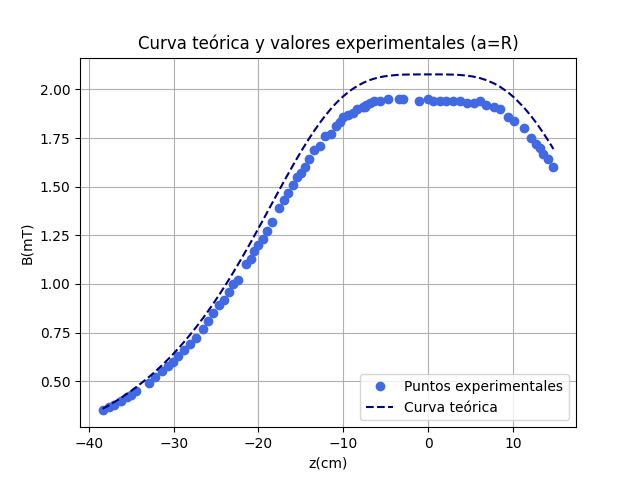
\includegraphics[width=0.85\linewidth]{Images/CurvaB1.png}
    \caption{Representación gráfica de los datos para $a=R$}
\end{figure}

Como hemos mencionado anteriormente, los valores de $z$ negativos son aquellos que se encuentran a la izquierda de las bobinas mientras que los positivos son aquellas medidas realizadas a la deerecha de las bobinas. En la gráfica se puede apreciar claramente que en los puntos interiores a las dos bobinas ($-10<z<10$) los valores del campo teórico y experimental difieren de forma notable. Esto se debe, como explicaremos al final de la sección, a un problema con la fuente de alimentación.

\subsubsection{$\mathbf{a=R/2}$}

Para el valor $a=R/2$ el procedimiento será el mismo, representaremos los valores del campo magnético teóricos y experimentales en una tabla, calcularemos su desviación cuadrática media y realizaremos una representación gráfica de los datos. En la siguiente tabla veremos los datos del campo magnético para diferentes valores de $z$:

\newpage

\begin{longtable}[t]{|c|c|c|c|c|c|}
    \hline
    $z \; (cm)$ & $B_{exp} \; mT$ & $B_T \; mT$ & $z \; (cm)$ & $B_{exp} \; mT$ & $B_T \; mT$ \\ \hline
    0.00     & 2.41 & 2.65 & -21.9 & 0.89 & 0.96 \\ \hline
    -1.2  & 2.40 & 2.64 & -23.6 & 0.77 & 0.84 \\ \hline
    -0.7  & 2.41 & 2.65 & -24.7 & 0.73 & 0.78 \\ \hline
    -2.4  & 2.38 & 2.61 & -26.9 & 0.62 & 0.66 \\ \hline
    -1.5  & 2.39 & 2.64 & -28.0 & 0.58 & 0.61 \\ \hline
    -2.4  & 2.37 & 2.61 & -29.2 & 0.54 & 0.56 \\ \hline
    -3.4  & 2.34 & 2.58 & -30.8 & 0.48 & 0.5  \\ \hline
    -4.1  & 2.32 & 2.54 & -32.5 & 0.43 & 0.45 \\ \hline
    -4.6  & 2.30 & 2.51 & -34.0 & 0.40 & 0.4  \\ \hline
    -5.3  & 2.25 & 2.47 & -35.2 & 0.37 & 0.37 \\ \hline
    -5.8  & 2.22 & 2.44 & -36.5 & 0.33 & 0.34 \\ \hline
    -6.3  & 2.17 & 2.4  & 1.3   & 2.41 & 2.64 \\ \hline
    -7.0  & 2.15 & 2.35 & 1.8   & 2.40 & 2.63 \\ \hline
    -8.2  & 2.06 & 2.24 & 2.5   & 2.39 & 2.61 \\ \hline
    -8.8  & 1.98 & 2.19 & 3.2   & 2.36 & 2.58 \\ \hline
    -9.5  & 1.94 & 2.12 & 4.0   & 2.32 & 2.55 \\ \hline
    -10.2 & 1.87 & 2.05 & 4.8   & 2.27 & 2.5  \\ \hline
    -11.0 & 1.82 & 1.97 & 5.5   & 2.24 & 2.46 \\ \hline
    -11.4 & 1.76 & 1.93 & 5.2   & 2.21 & 2.48 \\ \hline
    -12.0 & 1.71 & 1.86 & 6.9   & 2.14 & 2.35 \\ \hline
    -12.6 & 1.66 & 1.8  & 7.6   & 2.08 & 2.29 \\ \hline
    -13.1 & 1.60 & 1.75 & 8.3   & 2.03 & 2.23 \\ \hline
    -13.5 & 1.54 & 1.71 & 9.2   & 1.93 & 2.15 \\ \hline
    -14.2 & 1.48 & 1.63 & 10.0  & 1.88 & 2.07 \\ \hline
    -14.7 & 1.44 & 1.58 & 11.5  & 1.74 & 1.91 \\ \hline
    -15.5 & 1.37 & 1.5  & 12.7  & 1.62 & 1.79 \\ \hline
    -16.0 & 1.32 & 1.45 & 13.4  & 1.53 & 1.72 \\ \hline
    -16.9 & 1.25 & 1.37 & 14.5  & 1.45 & 1.6  \\ \hline
    -17.8 & 1.18 & 1.28 & 16.0  & 1.33 & 1.45 \\ \hline
    -19.3 & 1.07 & 1.15 & 17.5  & 1.21 & 1.31 \\ \hline
    -20.5 & 0.98 & 1.06 &       &      &      \\ \hline
    \caption{Valores teóricos y experimentales para $a=R/2$}
\end{longtable}

\newpage

A partir de estos datos debemos calcular la desviación cuadrática media entre los valores experimentales y teóricos del campo para determinar la exactitud de nuestras medidas. Para ello emplearemos la Ec.\ref{Desviación cuadrática media}, el resultado obtenido fue el siguiente:

\begin{equation}
    s = \frac{1}{N} \sqrt{\sum_{i=1}^{n} (B_{exp} - B_T)^2} = 0.091 \; mT
\end{equation}

En la siguiente figura podemos ver una representación gráfica de los valores experimentales y teóricos del campo magnético frente a $z$:

\begin{figure}[h!]
    \centering
    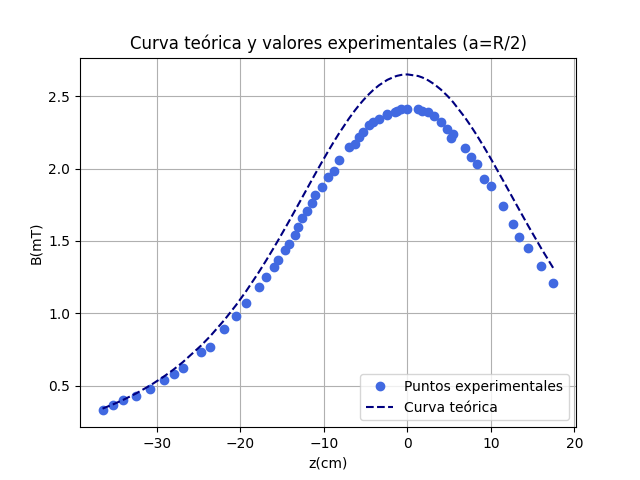
\includegraphics[width=0.85\linewidth]{Images/CurvaB2.png}
    \caption{Representación gráfica de los datos para $a=R/2$}
\end{figure}

Como en el apartado anterior, el valor de la curva teórica es notablemente mayor que el medido experimentalmente para valores de $z$ próximos al origen de coordenadas. Esto se debe, como explicaremos más detalladamente al final de la sección, a un problema con la fuente de alimentación, que no suministraba la suficiente corriente.

\subsubsection{$\mathbf{a=2R}$}

El procedimiento seguido será el mismo que en los apartados anteriores, representaremos en una tabla los valores teóricos y experimentales para diferentes valores de $z$, calcularemos la desviación cuadrática media entre los valores experimentales y teóricos y realizaremos una representación gráfica de los datos. En la siguiente tabla podemos ver los valores del campo magnético experimentales y teóricos en función de $z$:


\begin{longtable}[ht]{|c|c|c|c|c|c|}
    \hline
    $z \; (cm)$ & $B_{exp} \; (mT)$ & $B_T \; (mT)$ & $z \; (cm)$ & $B_{exp} \; (mT)$ & $B_T \; (mT)$ \\ \hline
    0     & 0.95 & 1.03 & -22.2 & 1.47 & 1.54 \\ \hline
    -0.9  & 0.95 & 1.03 & -22.8 & 1.46 & 1.52 \\ \hline
    -1.8  & 0.94 & 1.04 & -23.5 & 1.42 & 1.49 \\ \hline
    -3.   & 0.95 & 1.05 & -24.  & 1.40 & 1.47 \\ \hline
    -3.8  & 0.97 & 1.07 & -24.7 & 1.37 & 1.44 \\ \hline
    -4.5  & 1.00 & 1.08 & -25.5 & 1.34 & 1.4  \\ \hline
    -5.4  & 1.01 & 1.11 & -26.5 & 1.29 & 1.34 \\ \hline
    -6.   & 1.02 & 1.13 & -27.  & 1.26 & 1.31 \\ \hline
    -6.5  & 1.03 & 1.14 & -27.8 & 1.22 & 1.26 \\ \hline
    -7.2  & 1.06 & 1.17 & -28.5 & 1.17 & 1.21 \\ \hline
    -8.   & 1.08 & 1.2  & -29.5 & 1.11 & 1.15 \\ \hline
    -8.5  & 1.11 & 1.22 & -30.9 & 1.03 & 1.05 \\ \hline
    -9.   & 1.12 & 1.24 & -32.  & 1.00 & 0.98 \\ \hline
    -9.4  & 1.13 & 1.26 & -32.1 & 0.96 & 0.98 \\ \hline
    -10.  & 1.15 & 1.29 & -33.3 & 0.89 & 0.9  \\ \hline
    -10.6 & 1.19 & 1.31 & -34.5 & 0.82 & 0.83 \\ \hline
    -11.4 & 1.21 & 1.35 & -35.2 & 0.78 & 0.79 \\ \hline
    -11.9 & 1.23 & 1.37 & -36.  & 0.74 & 0.75 \\ \hline
    -12.4 & 1.26 & 1.4  & -36.8 & 0.70 & 0.7  \\ \hline
    -13.3 & 1.30 & 1.44 & -37.6 & 0.66 & 0.67 \\ \hline
    -14.1 & 1.34 & 1.47 & 0.5   & 0.95 & 1.03 \\ \hline
    -15.  & 1.37 & 1.5  & 1.    & 0.96 & 1.03 \\ \hline
    -15.6 & 1.39 & 1.52 & 1.5   & 0.96 & 1.03 \\ \hline
    -16.2 & 1.41 & 1.54 & 2.    & 0.97 & 1.04 \\ \hline
    -16.8 & 1.43 & 1.56 & 2.5   & 0.99 & 1.04 \\ \hline
    -17.5 & 1.45 & 1.57 & 3.    & 1.00 & 1.05 \\ \hline
    -18.2 & 1.46 & 1.58 & 3.5   & 1.01 & 1.06 \\ \hline
    -19.  & 1.48 & 1.58 & 4.    & 1.02 & 1.07 \\ \hline
    -19.8 & 1.48 & 1.58 & 4.5   & 1.03 & 1.08 \\ \hline
    -20.5 & 1.48 & 1.58 & 5     & 1.04 & 1.1  \\ \hline
    -21.5 & 1.47 & 1.56 &       &      &      \\ \hline
    \caption{Valores experimentales y teóricos del campo magnético para $a=2R$}
    \label{Datos a2R}
\end{longtable}



A partir de estos datos debemos calcular la desviación cuadrática media entre los valores experimentales y teóricos del campo para determinar la exactitud de nuestras medidas. Para ello emplearemos la Ec.\ref{Desviación cuadrática media}, el resultado obtenido fue el siguiente:

\begin{equation}
    s = \frac{1}{N} \sqrt{\sum_{i=1}^{n} (B_{exp} - B_T)^2} = 0.059 \; mT
\end{equation}

En la siguiente figura podemos ver representados gráficamente los valores experimentales y la curva teórica del campo magnético en función de $z$:

\begin{figure}[h!]
    \centering
    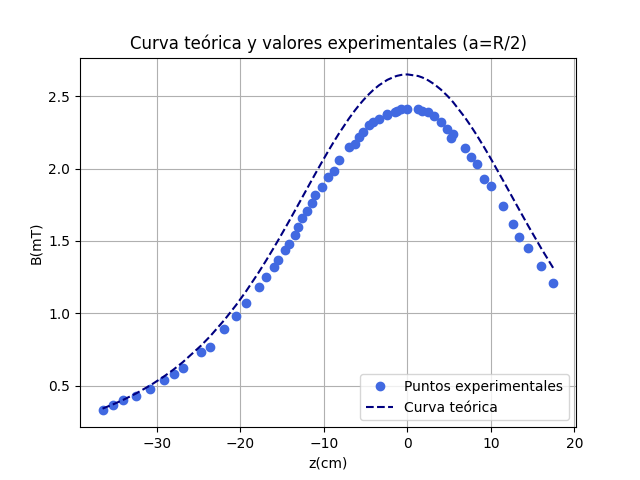
\includegraphics[width=0.85\linewidth]{Images/CurvaB2.png}
    \caption{Representación gráfica de los datos para $a=2R$}
\end{figure}

En la figura se puede observar claramente una discordancia notable entre la curva teórica y los valores experimentales, estando estos notablemente por debajo de lo esperado, especialmente para el intervalo $(-10<z<10)$. Este fenómeno se repitió en las tres medidas y se puede ver claramente en las tres gráficas que los valores experimentales están por debajo de lo esperado en este intervalo. El problema reside en la fuente de alimentación, que aunque estaba fijada en 3 A no suministraba tal intensidad de corriente, solía quedarse en unos 2,8 A. Este problema se nota especialmente en las zonas donde el campo es mayor y por tanto esta discordancia es más perceptible, coincidiendo en el intervalo ($-10<z<10$), que coincide con el interior y las proximidades de las bobinas. Para verificar que efectivamente el problema estaba en el problema con la intensidad de corriente hemos calculado una nueva curva teórica para cada una de las 3 situaciones con una intensidad de corriente de 2,8 A, en vez de los 3 a los que la máquina sospechamos que no llegaba. Gráficamente el resultado es el siguiente:

\begin{figure}[h!]
    \centering
    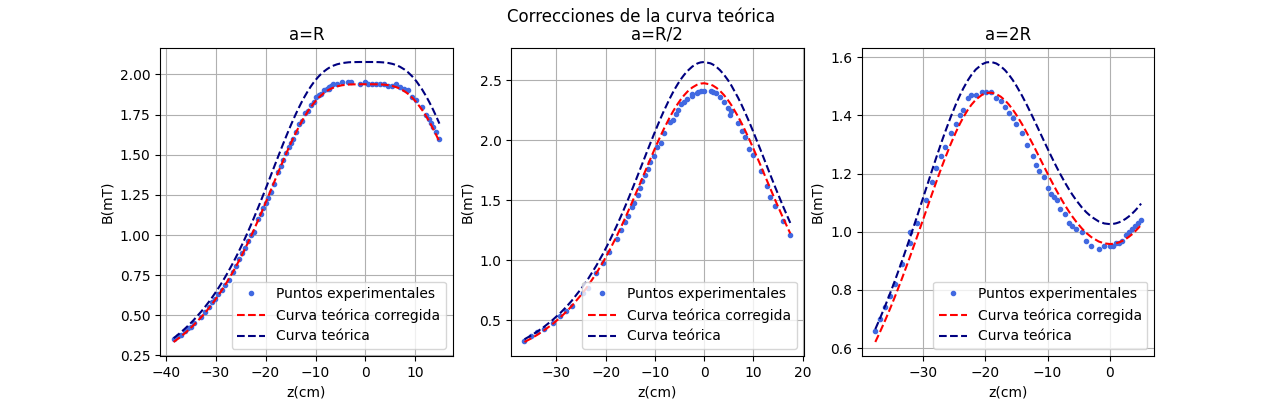
\includegraphics[width=1.25\linewidth]{Images/CurvasCorregidas.png}
    \caption{Curvas corregidas}
    \label{Curvas corregidas}
\end{figure}

Para comprobar matemáticamente nuestra hipótesis vamos a partir de que la intensidad en la Ec.\ref{Campo magnético} es un factor multiplicativo, por lo que el cociente $\frac{B_{T}}{B_{exp}}$ se debería mantener más o menos constante para todos los valores de $z$. Para comprobar esto vamos a calcular la media de estos cocientes y su desviación típica, que debería ser casi nula, según la siguiente expresión:

\begin{equation}
    \begin{gathered}
    \frac{B_{T}}{B_{exp}} = k \Rightarrow \overline{k} = \sum_i^{N} \frac{k_i}{N} \\
    s(k) = \sqrt{\frac{\sum_i^N (x_i-\overline{x})^2}{N-1}}
    \end{gathered}
\end{equation}

Si aplicamos estas fórmulas a los tres valores de $a$ obtenemos cocientes muy próximos a 1 y con desviaciones típicas muy pequeñas. Para $a=R$ la desviación típica es de $0.01$, para $a=R/2$ es de $0.02$ y para $a=2R$ es de $0.03$, que no superan el 3\% del valor de k, que se encuentra entre $1$ y $1,1$ en ambos casos. Por tanto, podemos concluir que, como la desviación típica es muy pequeña en todos los casos y es despreciable, el cociente $k$ es constante. Que este cociente sea constante reafirma nuestra afirmación de que la caída de intensidad de la fuente de alimentación provoca que los valores experimentales medidos estén por debajo de lo previsto.

\newpage

\subsection{Determinación de la permeabilidad magnética}

Como explicamos en la metodología, vamos a calcular la constante de permeabilidad magnética $\mu_0$ a partir de un ajuste por mínimos cuadrado de $B$ frente a $I$, que siguen la relación que se muestra en la Ec.\ref{Ec campo reducida}. Para ello tomamos 15 valores del campo magnético en el origen de coordenadas a diferentes valores de intensidades que representaremos en la siguiente tabla:

\begin{table}[h]
    \centering
    \begin{tabular}{|c|c|}
    \hline
    I (A) & B (mT) \\ \hline
    0,06  & 0,06   \\ \hline
    0,27  & 0,20    \\ \hline
    0,50   & 0,35   \\ \hline
    0,73  & 0,51   \\ \hline
    0,88  & 0,61   \\ \hline
    1,03  & 0,71   \\ \hline
    1,23  & 0,85   \\ \hline
    1,45  & 0,99   \\ \hline
    1,65  & 1,12   \\ \hline
    1,86  & 1,26   \\ \hline
    2,06  & 1,40    \\ \hline
    2,23  & 1,50   \\ \hline
    2,39  & 1,60    \\ \hline
    2,62  & 1,76   \\ \hline
    2,81  & 1,90    \\ \hline
    \end{tabular}
    \caption{Valores experimentales del campo magnético en función de la intensidad}
    \label{tab:my-table}
\end{table}

A partir de estos datos vamos a realizar un ajuste por mínimos cuadrados para ajustar los datos a una recta del tipo $(B=bI)$. Empleamos un ajuste simple sin término independiente porque a intensidad cero no hay campo magnético, este existe por la presencia de la corriente eléctrica circulando por la espira. Los valores obtenidos fueron los siguientes:

\begin{equation}
    \begin{gathered}
        b = 0.0006768 \; T\cdot A^{-1}\\
        s(b) = s(b) = 2.0 \cdot 10^{-6} \; T\cdot A^{-1} \\
        r = 0.99993 \\
        s = 1.3 \cdot 10^{-5}
    \end{gathered}
\end{equation}

En la siguiente figura podemos ver gráficamente el resultado del ajuste por mínimos cuadrados:

\begin{figure}
    \centering
    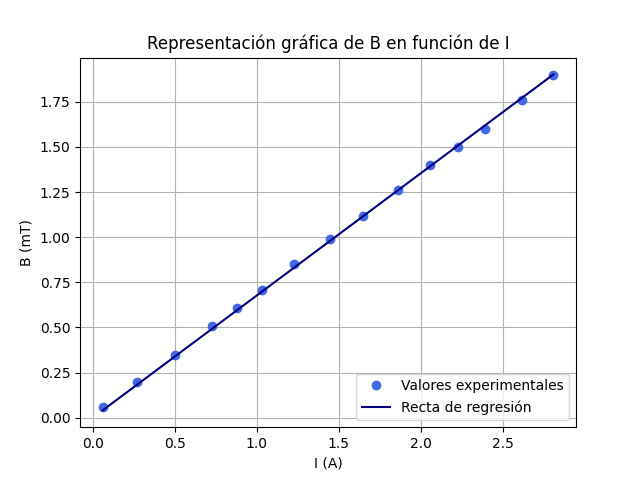
\includegraphics[width=0.85\linewidth]{Images/RegresionPermeabilidad.png}
    \caption{Valores experimentales y regresión de B frente a I}
\end{figure}

A partir de este resultado podemos calcular el valor de la permeabilidad con su incertidumbre aplicando la Ec.\ref{Permeabilidad magnética}, sustituyendo $a=R$ y la Ec.\ref{Incertidumbre permeabilidad}:

\begin{equation}
    \begin{gathered}
        \mu_0 = 1.2284 \cdot 10^{-6}\; T \cdot m \cdot A^{-1} \\
        s(\mu_0) = 3.7 \cdot 10^{-9}\; T \cdot m \cdot A^{-1}
    \end{gathered}
\end{equation}

Para el cálculo de la incertidumbre de $\mu_0$ empleamos la Ec.\ref{Incertidumbre permeabilidad}, como indicamos anteriormente, no obstante debemos notar que la única incertidumbre que participa es $s(b)$, ya que tomamos $\gamma$ como una constante con incertidumbre 0. La justificación matemática de esto es que el valor de $a=R$, a diferencia de los otros dos con los que trabajamos, no fue medido experimentalmente sino que venía determinado por las barras fijas que unían a las bobinas y que tenían una longitud igual a su radio. Es por esto que se decidió tomar este valor como constante y no dotarlo de incertidumbre, pues realmente no es ninguna medida, por lo que la incertidumbre de $\gamma$, que depende de la de $a$, es 0. Por tanto, la incertidumbre de $\mu_0$ viene dada por la siguiente expresión y tiene el valor mencionado anteriormente:

\begin{equation}
    s(\mu_0) = \frac{2R}{\gamma N} s(b)
\end{equation}

El valor real de la permeabilidad magnética depende del medio en el que nos encontremos, en el vacío tiene un valor de $\mu_0=4\pi\cdot 10^{-7} \; T \cdot m \cdot A^{-1}$, que es prácticamente el mismo valor que tiene en el aire, por lo que tomaremos ese valor como referencia. Si operamos el valor teórico obtenemos un resultado para la permeabilidad magnética de $1.2566 \cdot 10^{-6}\; T \cdot m \cdot A^{-1}$, que aunque no se encuentra en el rango de incertidumbre se encuentra muy próximo al valor determinado experimentalmente.

\section{Conclusión}

\subsection{Estudio del campo magnético axial creado por las bobinas}

En la primera parte los resultados experimentales se acercan en gran medida a los valores teóricos, especialmente si tenemos en cuenta la caída de intensidad de la fuente de alimentación. Como podemos ver en la Fig.\ref{Curvas corregidas}, una vez realizamos la corrección de las curvas a una intensidad de $2,8$ A los resultados experimentales se ajustan enormemente a la curva teórica. En la siguiente figura podemos ver los datos de los tres valores de $a$ con los que trabajamos:

\begin{figure}[h!]
    \centering
    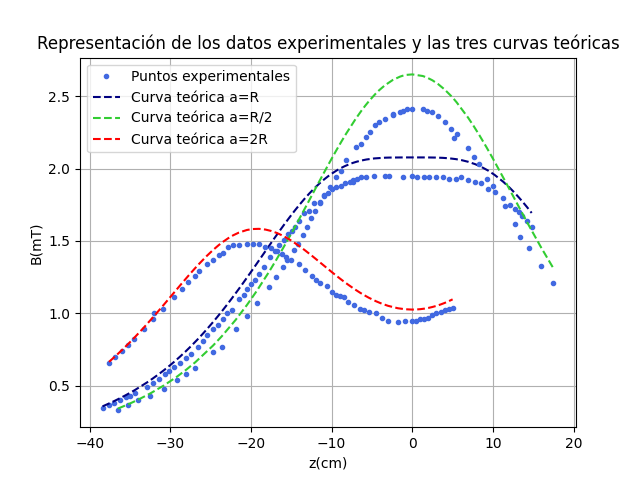
\includegraphics[width=0.95\linewidth]{Images/Tres curvas.png}
    \caption{Gráfica conjunta de las medidas experimentales y las curvas teóricas}
\end{figure}

\newpage

\subsection{Determinación de la permeabilidad magnética}

En la segunda parte de la práctica los resultados también se acercan en gran medida a lo esperado, algo que ya podíamos preveer por el buen coeficiente de regresión obtenido en el ajuste, y obtuvimos el siguiente valor para la constante:
\begin{table}[h!]
    \centering
    \begin{tabular}{c|c}
            $\mu_0$ & $4\pi\cdot 10^{-7} = 1.2566 \cdot 10^{-6} \; T \cdot m \cdot A^{-1}$ \\ \hline
            $\mu_{0exp}$ & $1.2284 \cdot 10^{-6} \pm 3.7 \cdot 10^{-9} \; T \cdot m \cdot A^{-1}$
    \end{tabular}
\end{table}

La diferencia entre ambos valores es ínfima y reafirma nuestras medidas realizadas durante toda la práctica, que se ajustan fielmente a la realidad.

\end{document}